\def\mytitle{Optimisation Assignment}
\def\myauthor{R.Radhika}
\def\contact{r170234@rguktrkv.ac.in}
\def\mymodule{Future Wireless Communication (FWC)}
\documentclass[10pt, a4paper]{article}
\usepackage[a4paper,outer=1.5cm,inner=1.5cm,top=1.75cm,bottom=1.5cm]{geometry}
\twocolumn
\usepackage[LGR,T1]{fontenc}
\usepackage[default]{gfsneohellenic}

\usepackage{setspace}
\usepackage{graphicx}
\graphicspath{{./images/}}
\usepackage[colorlinks,linkcolor={black},citecolor={blue!80!black},urlcolor={blue!80!black}]{hyperref}
\usepackage[parfill]{parskip}
\usepackage{lmodern}
\usepackage{tikz}
	\usepackage{physics}
%\documentclass[tikz, border=2mm]{standalone}
\usepackage{karnaugh-map}
\usepackage{tabularx}
\usetikzlibrary{calc}
\usepackage{amsmath}
\usepackage{amssymb}
\renewcommand*\familydefault{\sfdefault}
\usepackage{watermark}
\usepackage{lipsum}
\usepackage{xcolor}
\usepackage{listings}
\usepackage{float}
\usepackage{titlesec}
\providecommand{\mtx}[1]{\mathbf{#1}}
\titlespacing{\subsection}{1pt}{\parskip}{3pt}
\titlespacing{\subsubsection}{0pt}{\parskip}{-\parskip}
\titlespacing{\paragraph}{0pt}{\parskip}{\parskip}

\newcommand{\myvec}[1]{\ensuremath{\begin{pmatrix}#1\end{pmatrix}}}
\let\vec\mathbf
\lstset{
frame=single, 
breaklines=true,
columns=fullflexible
}

\title{\mytitle}
\author{\myauthor\hspace{1em}\\\contact\\FWC22066\hspace{6.5em}IITH\hspace{0.5em}\mymodule\hspace{6em}ASSIGN-6}
\date{}
\begin{document}
	\maketitle
	\tableofcontents
   \section{Problem}
 Find a point on the curve $x^2+2y^2=6$ whose distance from the line x+y=7 is minimum 
\section{Construction}
  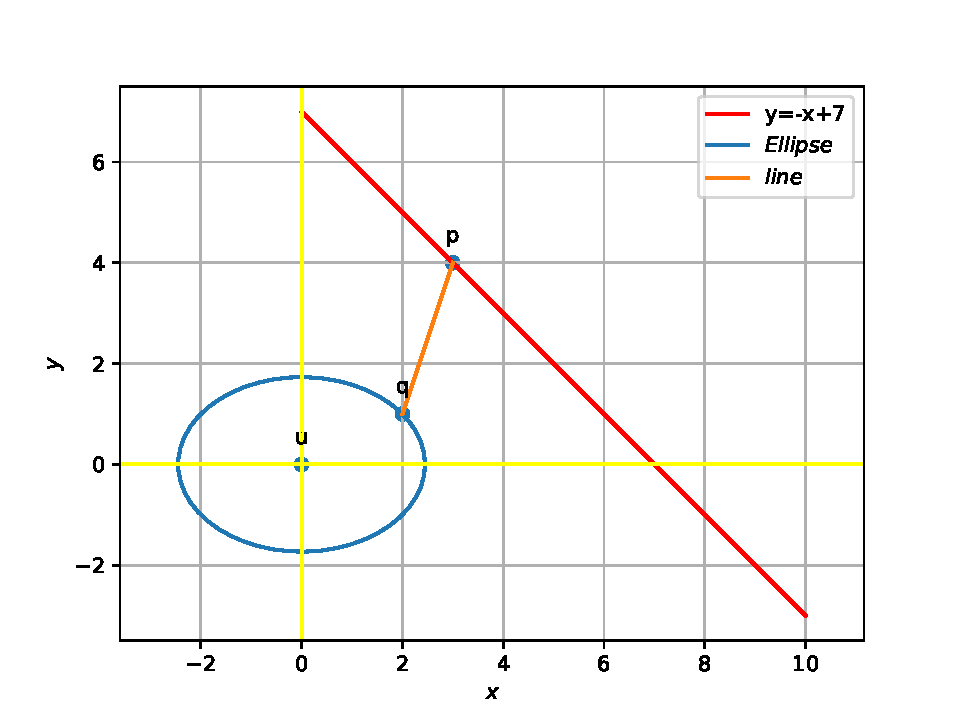
\includegraphics[scale=0.5]{ellipse.pdf}
  \begin{center}
  Figure of construction
  	\end{center}
given equation
\begin{align}
x^2+2y^2=6\\
\vec{x}+\vec{y}=7
\end{align}
we can write as\\
\begin{align}
\frac{x^2}{6}+\frac{y^2}{3}=1
\end{align}
  The dimensions of the figure is taken as below\\\\
{
\setlength\extrarowheight{2pt}
\centering
\begin{tabular}{|c|c|}
 \hline
 \textbf{Symbol}&\textbf{Value}\\
 \hline
 a&$\sqrt{6}$\\
 \hline
 b&$\sqrt{3}$\\
 \hline
\end{tabular}
}	
  \section{Solution}

Ellipse equation : \begin{align}
\frac{x^2}{6}+\frac{y^2}{3}=1
  \end{align}
The standard equation of the conics is given as :
\begin{align}
\vec{x}^{\top}\vec{V}\vec{x}+2\vec{u}^{\top}\vec{x}+f=0
\end{align}
For ellipse given that
\begin{equation}
\vec{u}=\myvec{0\\0}
\end{equation} 
From major axes equation of ellipse\\\\
\begin{equation}
a=\sqrt{\frac{\vec{u^T}\vec{V}^{-1}\vec{u}-f}{\lambda_1}}
\end{equation}
\begin{equation}
a=\sqrt{\frac{-f}{\lambda_1}}
\end{equation}
\begin{equation}
a^2=\frac{-f}{\lambda_1}
\end{equation}\\
\begin{equation}
\therefore \lambda_1=\frac{-f}{a^2}
\end{equation}
From minor axes equation of ellipse\\
\begin{equation}
b=\sqrt{\frac{\vec{u^T}\vec{V}^{-1}\vec{u}-f}{\lambda_2}}
\end{equation}
\begin{equation}
b=\sqrt{\frac{-f}{\lambda_2}}
\end{equation}
\begin{equation}
b^2=\frac{-f}{\lambda_2}
\end{equation}\\
\begin{equation}
\therefore \lambda_2=\frac{-f}{b^2}
\end{equation}
\begin{equation}
\therefore\lambda_1=-f/a^2 \;\;and\;\;\lambda_2=-f/b^2
\end{equation}

\begin{equation}
\vec{V}=\myvec{\lambda_1&0\\0&\lambda_2}
\end{equation}\\
\begin{equation}
\vec{V}=\myvec{-f/a^2&0\\0&-f/b^2}
\end{equation}\\
By substituting (16) in (4) we will get\\
\begin{equation}
\myvec{x&y}\myvec{-f/a^2&0\\0&-f/b^2}\myvec{x\\y}+f=0
\end{equation}\\
\begin{equation}
\myvec{x&y}\myvec{-f/a^2&0\\0&-f/b^2}\myvec{x\\y}=-f
\end{equation}\\
\begin{equation}
\myvec{x&y}\myvec{1/a^2&0\\0&1/b^2}\myvec{x\\y}=1
\end{equation}\\
\begin{equation}
\myvec{x&y}\myvec{1/6&0\\0&1/3}\myvec{x\\y}=1
\end{equation}
by using eq-14\\
$\therefore\lambda_1=1/a^2 \Rightarrow(1/6)\;\;and\;\;\lambda_2=-f/b^2 \Rightarrow(1/3)$
\begin{equation}
\vec{V}=\myvec{1/6&0\\0&1/3} and f=-1
\end{equation}
 For finding the point \\
\begin{equation}
\vec{q}=\vec{V}^{-1}(k\vec{n}-\vec{u})
\end{equation}
\begin{equation}
\vec{n}=\myvec{1\\1}
\end{equation}
And the intermediate parameters are given by\\
\begin{equation}
k=\pm\sqrt{\frac{\vec{u}^T\vec{v}^{-1}\vec{u}-f}{\vec{n}^T\vec{v}^{-1}\vec{n}}}
\end{equation}
substitute eq 5 and 21 in eq-23\\
we get $k=\pm\frac{1}{3}$\\
substitute k in eq-22 \\
yielding\\
\begin{equation}
\vec{q}=\myvec{2\\1}  \vec{m}=\myvec{-1\\1}, \vec{A}=\myvec{-7\\0},c=7
\end{equation}
equation of the line\\
$\vec{n^T}\vec{x}=c$

For finding the distance
\begin{equation}
d^2=\norm{\vec{x}-\vec{q}}^2
\end{equation}
The parametric equation of the line is
\begin{equation}
\vec{x}=\vec{A}+\lambda\vec{m}\\
\end{equation}
by 27 and 28 we can write as
\begin{equation}
d^2=\norm{(\vec{A}+\lambda\vec{m})-\vec{q}}^2
\end{equation}
yielding,\\
\begin{equation}
\lambda_{min}=-\frac{\vec{m^T}(\vec{A-q})}{\norm{\vec{m}}^2}
\end{equation}
substitute 26 in eq 30\\
yielding
$\lambda_{min}=-4$
\begin{equation}
\vec{x}=\myvec{-7\\0}+-4\myvec{-1\\1}
\end{equation}
yielding\\
$\vec{x}=\myvec{3\\4}$\\
substitute in eq 29 \\
yielding,
   
$\therefore{d}=\sqrt{10}=3.16$\\

$\therefore$The equation of ellipse is\\
\begin{equation}
\frac{x^2}{6}+\frac{y^2}{3}=1
\end{equation}
\section{Execution}
Verify the above problem in the following code.\\
\framebox{
\url{https://github.com/Radhikarkv/fwcproject.git}}	
\bibliographystyle{ieeetr}
\end{document}

